\begin{adjustbox}{width=\textwidth}
	\begin{tikzpicture}[every node/.style={inner sep=0,outer sep=0}]
		% Bilder
		\node [anchor=north west] (img1) at (0,0) {\includegraphics[frame,width=.31\textwidth]{05_ergebnisse/ergSichtpruefungDurchLichtstreuung/durchlichtAuswertungLichtstreuung/figures/gefärbtesBrillenglas2_rotiert_verbessert_Norm_LookUp}};
		\node [anchor=north west] (img2) at (0.345\textwidth,0) {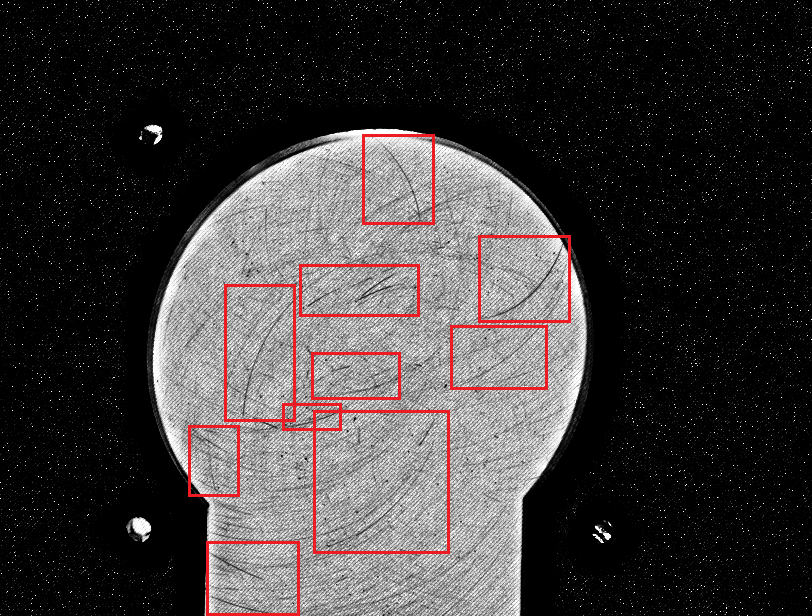
\includegraphics[frame,width=.31\textwidth]{05_ergebnisse/ergSichtpruefungDurchLichtstreuung/durchlichtAuswertungLichtstreuung/figures/polierfehler_ergebnis_verbessert}};
		\node [anchor=north west] (img3) at (0.69\textwidth,0) {\includegraphics[frame,width=.31\textwidth]{05_ergebnisse/ergSichtpruefungDurchLichtstreuung/durchlichtAuswertungLichtstreuung/figures/HS_Beschädigung_ergebnis_verbessert}};
		
		% Captions
		\node [below=0.2cm of img1] (cap1) {Brillenglas 1};
		\node [below=0.2cm of img2] (cap2) {Brillenglas 2};
		\node [below=0.2cm of img3] (cap3) {Brillenglas 3};			
	\end{tikzpicture}
\end{adjustbox}
\caption[Verbesserung der Ergebnisbilder]{Verbesserung der Ergebnisbilder. In Grün: Gravur der Brillenglaskennzeichnung. In Rot: Kratzer und ähnliche Beschädigungen der Oberfläche.\footnotemark}